% Dynamic Resonance Rooting: Calibrated Resonance and Lead--Lag Diagnostics
% for Complex Adaptive Systems.
%
% Revision of 25 November 2026. It supersedes the version of 25 September 2026
% (SSRN 5285993), kept beside this file as ssrn-5285993-sep2026.pdf. Its figures
% are taken from that PDF unchanged. The dependent-noise figure is drawn here
% with pgfplots from committed repository artifacts. Build with:  latexmk -pdf main.tex  (or pdflatex twice).
\documentclass[10pt,twocolumn,letterpaper]{article}

\usepackage[T1]{fontenc}
\usepackage[utf8]{inputenc}
\usepackage{mathptmx}
\usepackage[margin=0.72in,columnsep=0.24in]{geometry}
\usepackage{amsmath,amssymb,amsthm}
\usepackage{graphicx}
\usepackage{booktabs}
\usepackage{array}
\usepackage{xcolor}
\usepackage{enumitem}
\usepackage{caption}
\usepackage{titlesec}
\usepackage{pgfplots}
\pgfplotsset{compat=1.16}
\usepackage[hidelinks]{hyperref}

\captionsetup{font=footnotesize,labelfont=sc,labelsep=period}
\captionsetup[table]{position=top}
\renewcommand{\figurename}{Figure}
\titleformat{\section}{\centering\normalsize\scshape}{\Roman{section}.}{0.5em}{}
\titleformat{\subsection}{\normalsize\itshape}{\Alph{subsection}.}{0.5em}{}
\titlespacing*{\section}{0pt}{1.2ex plus .3ex}{0.8ex}
\titlespacing*{\subsection}{0pt}{1ex plus .2ex}{0.5ex}
\setlist{nosep,leftmargin=*}

\newtheorem{theorem}{Theorem}
\newtheorem{proposition}{Proposition}
\newtheorem{corollary}{Corollary}
\theoremstyle{definition}
\newtheorem{definition}{Definition}
\theoremstyle{remark}
\newtheorem{remark}{Remark}

\newcommand{\corr}{\operatorname{corr}}
\newcommand{\cov}{\operatorname{cov}}
\newcommand{\sd}{\operatorname{sd}}
\newcommand{\code}[1]{\texttt{#1}}
\newcommand{\ind}{\mathbf{1}}
\newcommand{\padj}{p^{\mathrm{adj}}}
\newcommand{\src}{ssrn-5285993-sep2026.pdf}

\begin{document}

\twocolumn[{%
\begin{center}
{\LARGE Dynamic Resonance Rooting: Calibrated Resonance and\\[2pt]
Lead--Lag Diagnostics for Complex Adaptive Systems\par}
\vspace{10pt}
{\large Christopher Woodyard\par}
{\small Vers3Dynamics, Bethesda, MD, USA\par}
\vspace{2pt}
{\footnotesize Revised 25 November 2026. Supersedes the version of 25 September 2026 (SSRN 5285993).\par}
\vspace{10pt}
\end{center}
\begin{minipage}{\textwidth}
\small
\noindent\textit{Abstract}---Dynamic Resonance Rooting (DRR) is an open-source
framework that summarizes multivariate time series with three diagnostics:
resonance (recurrent spectral modes), rooting (directed lead--lag edges), and
resonance depth (a composite rhythm score). We report four groups of results.
\emph{First}, we prove that for Gaussian signals every gain- and offset-invariant
score, resonance depth included, depends on the data only through the shape of
the power spectrum. This explains why depth ranks AR(1) noise at $\phi=0.9$
above a $-9$\,dB spectral line. We therefore redefine resonance as a spectral
line above the best-fitting monotone (``memory without rhythm'') continuum and
test it with a Monte Carlo spectral-excess statistic $\Lambda$. On 1,500
simulated rhythm-free series, $\Lambda$ holds its false-alarm rate between 0.037
and 0.067 at a nominal 0.05, where a fixed depth cutoff reaches 0.997, and it
detects a $-9$\,dB line in AR(0.9) noise in 80\% of trials. \emph{Second}, we
derive in closed form that lagged correlation makes a target appear to lead its
own source with correlation $c\phi^{\ell+d}$, and show that channel-wise
prewhitening removes the artifact in population. At $\phi=0.9$ and 512 samples,
prewhitened rooting recovers a 0.3 coupling at its true lag in 300 of 300
systems, against 40\% for the current test. \emph{Third}, we map where the
circular-shift surrogate null holds. Its family-wise error is 0.048--0.060 on
fractional Gaussian noise up to Hurst exponent 0.95 and 0.055 under GARCH(1,1),
but it reaches 0.28 on random walks, 0.145 on independent coherent oscillators
at a shared frequency, and 0.150 on independent series that share an amplitude
trend. A seam ablation points to the cause of the oscillator failure.
\emph{Fourth}, we report three preregistered external tests. None supported its
claim. On NOAA quasi-biennial-oscillation winds the holdout false-alarm rate was
0.272 against a 0.05 tolerance. In a daily cryptocurrency-return holdout, DRR
features improved squared error by 0.34\%, short of the registered 1\% and not
significant after correction. In a lead--lag breakdown study, signed correlation
detected reversals faster. Every number is read from scripts or artifacts pinned
to configuration hashes. DRR outputs are diagnostics, not causal, policy, or
supervisory conclusions.

\smallskip
\noindent\textit{Index Terms}---complex adaptive systems, surrogate data,
red-noise null, spectral line detection, lead--lag analysis, prewhitening,
long memory, family-wise error, preregistration, negative results, model-risk
review.
\end{minipage}
\vspace{14pt}
}]

\section{Introduction}

Complex adaptive systems (CAS), such as climate modes, ecosystems, markets, and
supervised financial institutions, leave traces that are rhythmic, lagged, and
changeable before they can be explained mechanistically \cite{holland,mitchell}.
Tools that look for early warnings in such traces have a well-documented
weakness: they find rhythms and leads that are not there. Rising
autocorrelation, spectral reddening, and apparent lead--lag structure are all
generic consequences of memory \cite{ditlevsen,boettiger}. A framework that
reports ``a resonance'' or ``a root'' is only as useful as its false-alarm rate.

DRR is public research software built around calibration studies,
specification tests, and preregistered external comparisons \cite{drr}. The
first version of this paper started from three uncomfortable facts, all
documented in the repository. Resonance depth cannot tell red noise from a weak
resonance. The lead--lag test reports the target leading its own source when
channels have memory. The one external test failed its preregistered
false-alarm tolerance.

Since then the repository has added five studies, each with its hypotheses or
decision rule fixed before scoring. Two map the validity of the surrogate null
under long memory, heavy tails, coherent oscillation, and shared
nonstationarity. One compares rooting with prewhitening-style baselines. Two
are new preregistered external tests on market data. Both external tests
failed. This revision adds those results and updates the evidence ledger. The
thesis is unchanged: a diagnostic framework earns trust through calibrated
error rates and published failures, not through breadth.

The contributions are:
\begin{enumerate}[label=\textbf{C\arabic*}]
\item \emph{A spectral-sufficiency theorem} (Thm.~\ref{thm:suff}). Under
Gaussianity, depth and every other affine-invariant score are functionals of
spectral shape. The theorem explains the red-noise confusion, predicts that
phase-randomized placebos have no power, and fixes the only well-posed null for
resonance: a spectral one.
\item \emph{A falsifiable definition of resonance and a calibrated test.}
Resonance is a spectral line above the best monotone continuum, the class of
continua that memory alone can produce. The spectral-excess test $\Lambda$ and
a calibrated depth score $D^*$ are evaluated on 16 simulated families
(Section~\ref{sec:calres}).
\item \emph{Closed-form analysis of lagged-correlation rooting under memory},
and a prewhitened rooting operator that provably removes the reverse-lead
artifact. Size, power, and lag localization are compared with the v2 test and a
Granger F-test (Section~\ref{sec:calroot}).
\item \emph{The validity region of the surrogate null.} Measured family-wise
error under fractional Gaussian noise, GARCH, random walks, coherent
oscillators, and shared trends, with an ablation that traces the oscillator
failure to the circular-shift seam (Section~\ref{sec:nulls}).
\item \emph{Three complete negative results.} Preregistered tests on
stratospheric winds and on two market tasks, none of which supported its claim,
reported in full with every comparison (Section~\ref{sec:external}).
\item \emph{An evidence ledger.} A claim-status discipline (supported,
not\_supported, withdrawn) in which every number in this paper traces to a
hash-pinned script or artifact (Section~\ref{sec:ledger}, Appendix).
\end{enumerate}

\section{Background and Related Work}

\textit{Surrogate data.} Surrogate tests compare a statistic with its
distribution under a null model realized by resampling. Examples include
phase-randomized (Fourier) surrogates for linear Gaussian nulls,
amplitude-adjusted variants, and time shifts for independence
\cite{theiler,schreiber,lancaster}. Their validity rests on the resampling
scheme's invariance under the null, which we make precise for rooting in
Prop.~\ref{prop:exact}.

\textit{Red-noise nulls.} Climate science has long tested spectral peaks against
a fitted AR(1) ``red-noise'' background rather than white noise
\cite{gilman,mannlees,torrence}. Burg's maximum-entropy principle identifies
AR($p$) as the least-structured Gaussian process that matches $p+1$
autocovariances \cite{burg}. Monotone spectral densities can be estimated
nonparametrically by isotonic regression \cite{barlow,anevski}.

\textit{Long memory and nonstationarity.} Fractional Gaussian noise (fGn) with
Hurst exponent $H>1/2$ has autocorrelations that decay as a power law
\cite{mandelbrot}, and it can be simulated exactly by circulant embedding
\cite{daviesharte}. GARCH processes are serially uncorrelated but dependent in
their squares \cite{bollerslev}. Independent random walks produce large
spurious correlations \cite{grangernewbold}.

\textit{Lead--lag and causality.} Granger causality tests whether a source's
past improves prediction of a target beyond the target's own past
\cite{granger}. Cross-correlating raw autocorrelated series inflates spurious
association \cite{bartlett}. Prewhitening, i.e., cross-correlating innovations,
is the classical remedy \cite{boxjenkins,haugh}. Modern causal discovery
conditions on autocorrelation and on confounders explicitly \cite{pcmci}.
Family-wise error across many edges and lags is controlled by max-statistic
resampling \cite{westfall}. Phase synchronization generalizes lead--lag
coupling to $n{:}m$ frequency ratios \cite{rosenblum}.

\textit{Early warning and preregistration.} Early-warning indicators for
critical transitions \cite{scheffer,dakos} are vulnerable to false alarms and to
post hoc tuning \cite{ditlevsen,boettiger}. Preregistration fixes hypotheses,
data, and decision rules before outcomes are seen \cite{nosek}. In model-risk
practice, conceptual soundness, ongoing monitoring, and outcomes analysis are
the core elements of validation \cite{sr117}.

\section{The DRR Operators}

Let $X\in\mathbb{R}^{T\times n}$ hold $T$ observations of $n$ observables, and
let $x_j$ be column $j$.

\textit{Resonance depth} (\code{drr\_composite\_v2}). For a window $w$ of one
trace, DRR selects a target frequency $\hat f_0$, the peak of the Welch spectrum
\cite{welch} refined by log-parabolic interpolation, and scores
\begin{equation}\label{eq:depth}
D=\operatorname{clip}_{[0,1]}\bigl(0.35\,S+0.25\,P+0.25\,C+0.15\,A\bigr).
\end{equation}
Here $S$ is the Welch power within one bin of $\hat f_0$ over total power. $P$
is the mean of $\exp\{-[(\hat f^{(k)}-\hat f_0)/\delta]^2\}$ over sub-windows
$k$, with $\delta$ one bin of the sub-window spectrum. $C=\bigl|\overline{\exp\{i(\theta_t-2\pi \hat f_0 t)\}}\bigr|$,
where $\theta_t$ is the Hilbert phase \cite{gabor} and the bar denotes a time
average. $A=1-\sd(a_t)/\bar a$, where $a_t$ is the Hilbert envelope. The
current composite corrects two defects of an earlier implementation. First,
$\delta$ was floored at 0.5 in the caller's units, so monthly or 1\,Hz series
always looked persistent. Second, an unrefined $\hat f_0$ made $C$ depend on the
FFT grid. Property tests confirm invariance to time unit, grid position, gain,
and offset \cite{drr}.

\textit{Rooting.} For an ordered pair $(i,j)$ and lags $\ell=1,\dots,L$,
\begin{equation}\label{eq:root}
R_{ij}=\max_{1\le \ell\le L}\bigl|\hat\rho_{ij}(\ell)\bigr|,\qquad
\hat\rho_{ij}(\ell)=\widehat{\corr}(x_{i,t-\ell},x_{j,t}),
\end{equation}
and the maximizing lag is reported as the edge lag. Significance uses
surrogates $X^{(b)}$ in which every column is circularly shifted by an
independent offset, and the max statistic $M=\max_{i\ne j}R_{ij}$. The adjusted
$p$-value is
\begin{equation}\label{eq:padj}
\padj_{ij}=\frac{1+\#\{b\le B: M^{(b)}\ge R_{ij}\}}{B+1}.
\end{equation}
A heuristic gate ($R_{ij}>\mu+\sigma$ of the score matrix) preselects
candidates. It can hide edges but cannot add them. The package also offers a
phase-randomization null, which keeps each series' periodogram and draws new
phases \cite{theiler}. Fig.~\ref{fig:pipeline} shows the v3 pipeline built from
these operators.

\begin{figure}[t]
\centering
\includegraphics[page=2,trim=312 563 52 52,clip,width=\columnwidth]{\src}
\caption{DRR v3. Blue boxes are the calibrated operators introduced here. Every
output enters an evidence ledger with a machine-readable claim status before
any interpretation, and nothing crosses the review boundary without
independent validation.}
\label{fig:pipeline}
\end{figure}

\section{Theory}

\subsection{Validity of the circular-shift max-statistic test}

\begin{proposition}[Exactness under circular stationarity]\label{prop:exact}
Suppose that under $H_0$ the $n$ coordinate processes are mutually independent
and each is circularly stationary on $\mathbb{Z}_T$, i.e., its law is invariant
under cyclic rotation. Let $G=\mathbb{Z}_T^n$ act by independent rotations of
the columns, let $g_1,\dots,g_B$ be drawn i.i.d.\ uniformly from $G$, and set
$X^{(b)}=g_bX$. Then $\Pr\{\exists\, i\ne j:\padj_{ij}\le\alpha\}\le\alpha$ for
every $\alpha\in(0,1)$.
\end{proposition}
\begin{proof}
Under $H_0$ the law of $X$ equals the law of $gX$ for every $g\in G$, because
independent columns rotated independently keep their joint law. For any
statistic, the Monte Carlo $p$-value
$(1+\#\{b:M(g_bX)\ge M(X)\})/(B+1)$ is then valid \cite{hemerik,lehmann}. If
some $\padj_{ij}\le\alpha$, then, because $R_{ij}\le M(X)$,
$\#\{b:M^{(b)}\ge M(X)\}\le\#\{b:M^{(b)}\ge R_{ij}\}$, so the $p$-value of $M$
is also $\le\alpha$. Hence the family-wise error is at most $\alpha$.
\end{proof}

\begin{remark}\label{rem:seam}
The implementation departs from Prop.~\ref{prop:exact} in two ways. Real
series are stationary rather than circularly stationary, so rotation creates a
seam. Offsets are drawn uniformly from the subset of $G$ whose pairwise
circular separations exceed $L$, which avoids surrogates that re-create the
observed alignment. Neither departure is covered by the proposition, so their
effect is measured. Family-wise error is 0.040--0.062 across AR(1)
coefficients 0--0.97 (Table~\ref{tab:size}). Section~\ref{sec:nulls} shows
where the seam does matter: coherent oscillators. There, removing the seam
correction from the related phase test raises its false-alarm rate from 0.040
to 0.170. The proposition also explains
a bug the calibration study found. An earlier generator split the slack
between offsets with a multinomial draw. This concentrated surrogates near
evenly spaced configurations, broke the uniformity the proof needs, and raised
the white-noise family-wise error to 0.14. Unit tests of surrogate shape could
not see this defect. Only a size study could.
\end{remark}

\subsection{What resonance depth can know}

\begin{theorem}[Spectral sufficiency]\label{thm:suff}
Let $x=(x_1,\dots,x_T)$ be a sample from a stationary Gaussian process with mean
$\mu$ and spectral density $f$, and let $D:\mathbb{R}^T\to\mathbb{R}$ be
measurable with $D(ax+b\mathbf{1})=D(x)$ for all $a>0$, $b\in\mathbb{R}$. Then
the law of $D(x)$ depends on $(\mu,f)$ only through the spectral shape
$f/\!\int f$.
\end{theorem}
\begin{proof}
$x\sim\mathcal{N}(\mu\mathbf{1},\Sigma)$ with
$\Sigma_{st}=\gamma(s-t)=\int e^{i\lambda(s-t)}f(\lambda)\,d\lambda$
\cite{brockwell}. Put $\sigma^2=\gamma(0)=\int f$ and $z=(x-\mu\mathbf{1})/\sigma$.
Then $z\sim\mathcal{N}(0,\Sigma/\sigma^2)$, whose covariance is determined by
$f/\!\int f$, and $D(x)=D(\sigma z+\mu\mathbf{1})=D(z)$.
\end{proof}

\begin{corollary}\label{cor:suff}
(a) Gaussian processes with proportional spectra give identically distributed
depth. For Gaussian signals, $C$ (``phase coherence'') carries no information
beyond spectral bandwidth. (b) Fourier surrogates preserve the periodogram and
randomize phases \cite{theiler}. For Gaussian input they sample, approximately,
the input's own law, so a depth placebo against them has power near its size.
The repository's measured depth change of about 0.005 under phase
randomization \cite{drr} is therefore the predicted outcome, not a defect of
the placebo. (c) Any well-posed null hypothesis for depth is a statement about
the spectrum.
\end{corollary}

Thm.~\ref{thm:suff} turns a vague notion (``persistent modal structure'') into
a sharp question: which spectra count as having no rhythm? Memory alone
produces spectra that are monotone in frequency. White noise, AR(1) at any
$\phi$, and sums of positively correlated AR(1) processes with white noise are
all monotone. An interior spectral maximum, from a deterministic line or a
stochastic oscillator, is exactly what memory cannot produce.

\begin{definition}[Resonance, v3]\label{def:res}
A trace exhibits a resonance at level $\alpha$ if a level-$\alpha$ test rejects
$H_{\mathrm{mono}}$: the trace is a stationary Gaussian process with a monotone
spectral density.
\end{definition}

\textit{Spectral-excess statistic.} Let $I_k$ be the periodogram of the demeaned
trace at interior Fourier bins $k=1,\dots,\lfloor T/2\rfloor-1$. Let $m_k$ be
the $L^2$ isotonic projection of $\log I_k$ onto non-increasing or
non-decreasing sequences, whichever fits better. Set
$\hat S_k=\exp(m_k+\gamma_E)$, where Euler's constant $\gamma_E$ corrects the
mean of the log of an Exp(1) ordinate. Then
\begin{equation}\label{eq:lambda}
\Lambda=\max_k I_k/\hat S_k,
\end{equation}
and $p$ is computed from $B$ Gaussian surrogates with spectrum $\hat S$, each
refitted, so the null includes the fitting step. Fitting on the log scale
bounds the pull a single line exerts on its own null. A line 25 times the local
continuum moves one log-ordinate by about $\ln 25\approx3.2$, against a noise
standard deviation of $\pi/\sqrt6\approx1.28$.

\textit{Calibrated depth.} We also report $D^*$, the depth $p$-value and
$z$-score against a fitted null. We use two nulls: the AR(1) process matched to
the sample lag-1 autocorrelation, which is Burg's maximum-entropy process
\cite{burg}, and a Gaussian process with the isotonic periodogram fit (the
linear-scale analog of $\hat S$). $D^*$ keeps depth's descriptive meaning and
gives it a reference frame. $\Lambda$ is the test.

\subsection{Why lagged correlation reverses leads}

Consider the design of the repository's calibration study. The source is a
unit-variance AR(1), $x_t=\phi x_{t-1}+\sqrt{1-\phi^2}\,\varepsilon_t$, with
i.i.d.\ standard normal $\varepsilon$. The target is $y_t=c\,x_{t-d}+s\,u_t$,
where $s=\sqrt{1-c^2}$ and $u$ is an independent unit-variance AR(1) with the
same $\phi$ and innovations $\eta$.

\begin{proposition}[Raw and prewhitened correlations]\label{prop:rev}
(i) \emph{Raw.} $\corr(x_{t-\ell},y_t)=c\,\phi^{|\ell-d|}$ in the forward
direction, and
\begin{equation}\label{eq:rev}
\corr(y_{t-\ell},x_t)=c\,\phi^{\ell+d},\qquad \ell\ge1,
\end{equation}
in the reverse direction. (ii) \emph{Prewhitened.} $y$ is itself AR(1) with
coefficient $\phi$ and innovation $\sqrt{1-\phi^2}\,(c\,\varepsilon_{t-d}+s\,\eta_t)$.
The innovation cross-correlation is therefore $c\cdot\ind\{\ell=d\}$ in the
forward direction and 0 in reverse at every $\ell\ge1$. (iii) \emph{Null
width.} For independent series,
$\sd(\hat\rho)\approx\sqrt{(1+\phi^2)/[T(1-\phi^2)]}$ on raw series
\cite{bartlett} and $1/\sqrt T$ on innovations. Prewhitening multiplies the
noncentrality of the true edge by $\kappa(\phi)=\sqrt{(1+\phi^2)/(1-\phi^2)}$.
\end{proposition}
\begin{proof}
(i) Covariances follow from $\cov(x_s,x_t)=\phi^{|s-t|}$ and independence of
$u$. (ii) $y_t-\phi y_{t-1}=c(x_{t-d}-\phi x_{t-d-1})+s(u_t-\phi u_{t-1})$, which
is an innovation sequence of variance $1-\phi^2$. (iii) is Bartlett's formula
$\operatorname{var}\hat\rho\approx T^{-1}\sum_h\rho_{xx}(h)\rho_{yy}(h)$.
\end{proof}

More generally, whenever $x$ has a correctly specified AR representation and
receives no feedback from $y$, $x$'s innovation at $t$ is independent of all
data up to $t-1$. It is therefore uncorrelated with any function of
$y_{\le t-\ell}$, and the reverse lead vanishes in population.
Table~\ref{tab:prop2} checks every prediction of Prop.~\ref{prop:rev} against
$4\times10^5$-sample simulations and against the Monte Carlo study. For
narrowband sources the raw failure is worse. A stochastic oscillator has
$\rho_{xx}(h)\approx r^h\cos(2\pi f_0h)$, so the forward lags $d\pm1$ nearly tie
with the true lag $d$, and raw rooting localizes the lag poorly
(Table~\ref{tab:memory}). Long memory is a harder case: fGn has no finite AR
representation, so a finite-order prewhitening filter can only approximate its
innovations. Section~\ref{sec:nulls} measures the raw operator under fGn. The
prewhitened operator has not yet been tested there.

\begin{table}[t]
\centering\footnotesize
\caption{Predictions of Prop.~\ref{prop:rev} ($c=0.3$, $d=2$, $T=512$) against
simulation. $z$ denotes the noncentrality of the true edge.}
\label{tab:prop2}
\begin{tabular}{@{}lccc@{}}
\toprule
 & $\phi=0.5$ & $\phi=0.9$ & $\phi=0.97$\\
\midrule
Reverse corr.\ $c\phi^3$, predicted & 0.037 & 0.219 & 0.274\\
\quad simulated ($T=4\times10^5$) & 0.038 & 0.228 & 0.276\\
Prewhitened reverse corr., predicted & 0 & 0 & 0\\
\quad simulated & $-0.000$ & 0.002 & $-0.000$\\
Raw $z=c\sqrt T/\kappa(\phi)$ & 5.26 & 2.20 & 1.18\\
Prewhitened $z=c\sqrt T$ & 6.79 & 6.79 & 6.79\\
Raw exact-lag recovery (measured) & 0.990 & 0.403 & 0.120\\
Prewhitened (measured) & 1.000 & 1.000 & 1.000\\
\bottomrule
\end{tabular}
\end{table}

\section{Calibration Study: Rooting}\label{sec:calroot}

\textit{Design.} All settings were frozen in a configuration file (SHA-256
\code{57d5ea78\ldots}) before the first run. Each system has 512 samples, lags
run from 1 to 4, and each test uses 99 surrogates, $\alpha=0.05$, and
max-statistic correction. Prewhitening fits an AR($p$) per channel with
$p\le10$ chosen by AIC \cite{akaike}. Three procedures see identical data: (1)
v2 rooting on raw series; (2) v3 prewhitened rooting, which is the same test on
innovations; and (3) a pairwise Granger F-test with AIC-chosen own lags, source
lags 1--4, and Bonferroni correction over ordered pairs. Granger's reported lag
is the source lag with the largest coefficient. That rule is ours, not part of
the test, so we score Granger on edge detection at any lag. Intervals are
Wilson 95\% intervals \cite{wilson}.

\begin{table}[t]
\centering\footnotesize
\caption{Size. Family-wise error (any significant edge) on three independent
channels, 400 systems per row, nominal $\alpha=0.05$. Brackets: Wilson 95\%
intervals.}
\label{tab:size}
\setlength{\tabcolsep}{3.2pt}
\begin{tabular}{@{}llll@{}}
\toprule
Null & v2 raw & v3 prewhitened & Granger\\
\midrule
AR(1), $\phi=0$ & .062 [.043,.091] & .065 [.045,.094] & .048 [.031,.073]\\
AR(1), $\phi=0.5$ & .040 [.025,.064] & .065 [.045,.094] & .058 [.039,.085]\\
AR(1), $\phi=0.9$ & .048 [.031,.073] & .058 [.039,.085] & .050 [.033,.076]\\
AR(1), $\phi=0.97$ & .062 [.043,.091] & .040 [.025,.064] & .058 [.039,.085]\\
AR(2) osc., $r=.95$ & .058 [.039,.085] & .030 [.017,.052] & .050 [.033,.076]\\
\bottomrule
\end{tabular}
\end{table}

\begin{table}[t]
\centering\footnotesize
\caption{Memory and oscillators. Coupling $c=0.3$ at lag 2; 300 systems per
row. ``Exact'': true edge at true lag. ``Rev.'': target reported leading
source.}
\label{tab:memory}
\setlength{\tabcolsep}{3.5pt}
\begin{tabular}{@{}lcccccc@{}}
\toprule
 & \multicolumn{2}{c}{v2 raw} & \multicolumn{2}{c}{v3 prewhitened} & \multicolumn{2}{c}{Granger}\\
\cmidrule(lr){2-3}\cmidrule(lr){4-5}\cmidrule(l){6-7}
Channel memory & Exact & Rev. & Exact & Rev. & Any lag & Rev.\\
\midrule
AR(1) $\phi=0$ & 1.000 & .000 & 1.000 & .000 & 1.000 & .013\\
AR(1) $\phi=0.5$ & .990 & .013 & 1.000 & .003 & 1.000 & .010\\
AR(1) $\phi=0.8$ & .720 & .097 & .997 & .000 & 1.000 & .003\\
AR(1) $\phi=0.9$ & .403 & .120 & 1.000 & .000 & 1.000 & .003\\
AR(1) $\phi=0.97$ & .120 & .107 & 1.000 & .003 & 1.000 & .010\\
AR(2) $r=.95$ osc. & .153 & .023 & 1.000 & .007 & .997 & .017\\
\bottomrule
\end{tabular}
\end{table}

\textit{Size.} All three procedures hold nominal family-wise error on every
null, including independent narrowband oscillators at a shared frequency, which
strongly cross-correlate by chance (Table~\ref{tab:size}). Every Wilson interval
covers 0.05. The v2 rows share seeds with the committed calibration study and
reproduce its values exactly.

\textit{Memory.} Table~\ref{tab:memory} and Fig.~\ref{fig:rooting} show the
central rooting result. As memory rises from $\phi=0.5$ to 0.97, v2 exact
recovery falls from 0.990 to 0.120 and reverse edges rise to 10--12\%. This
matches Prop.~\ref{prop:rev}: the raw noncentrality collapses from 5.3 to 1.2
while the reverse correlation approaches the true one. Prewhitened rooting
recovers the edge at its true lag in 1,499 of 1,500 systems across
$\phi\in\{0,\dots,0.97\}$, with at most 0.3\% reverse edges. The failure grows
with coupling strength. At $\phi=0.9$ and $c=0.5$, v2 reports the reverse edge in
51.0\% of systems, because the artifact scales with $c$. Prewhitening reports
it in none. On coupled stochastic oscillators, v2 finds the edge at any lag in
only 30.3\% of systems and at the true lag in 15.3\%. v3 finds it at the true
lag in all 300.

\textit{Against Granger.} In this linear-Gaussian design, prewhitened rooting
and the Granger F-test detect edges equally well: power at $\phi=0.9$ is 0.207
vs.\ 0.197 at $c=0.1$ and 0.890 vs.\ 0.883 at $c=0.2$. This is expected, since
both condition on the target's own past. What rooting adds is a
resampling-based family-wise guarantee across all edges and lags, with a
localized lag. We do not claim that DRR outperforms Granger. The claim is
narrower: the v2 lead--lag operator was the wrong estimator under memory, and
v3 matches the conventional benchmark.

\begin{figure*}[t]
\centering
\includegraphics[page=5,trim=40 580 46 46,clip,width=\textwidth]{\src}
\caption{Rooting under memory. (a) The v2 test loses the true edge as memory
grows; prewhitening and Granger do not. (b) The v2 reverse-edge artifact follows
Eq.~\eqref{eq:rev}; prewhitening removes it. (c) At $\phi=0.9$, v3 and Granger
have indistinguishable power (0.890 vs.\ 0.883 at $c=0.2$). The v2 test detects a
0.5 coupling in 91\% of systems but also reports the reverse edge in 51\%. Bars:
Wilson 95\% intervals; 300 systems per point.}
\label{fig:rooting}
\end{figure*}

\begin{figure*}[t]
\centering
\includegraphics[page=5,trim=40 343 46 246,clip,width=\textwidth]{\src}
\caption{Resonance testing. (a) A fixed depth cutoff is a red-noise detector: its
false-alarm rate climbs to 0.997 as memory grows. The AR(1)-calibrated $D^*$
holds size on AR(1) but fails (0.617) when white measurement noise is added,
which is misspecification. The isotonic $D^*$ and $\Lambda$ hold size on all five
nulls. (b) Only $\Lambda$ detects lines in red backgrounds. Broad oscillators
($r\le0.9$) are nearly indistinguishable from a monotone continuum at $T=512$ by
any method.}
\label{fig:resonance}
\end{figure*}

\section{Calibration Study: Resonance}\label{sec:calres}

\textit{Design.} Each series has 512 samples, a depth window of 256, and 99
null draws per test. There are 300 draws per null family and 200 per
alternative. Lines sit at 0.0625 cycles/sample. The procedures are: the v2
depth with a fixed cutoff of 0.227, the 95th percentile under white noise from
the committed artifact; $D^*$ with the AR(1) null; $D^*$ with the isotonic null;
and $\Lambda$.

\begin{table}[t]
\centering\footnotesize
\caption{Rejection rates. Top: rhythm-free nulls (false alarms; nominal .05).
Bottom: resonances (power). 300 (null) or 200 (alternative) series per row.}
\label{tab:res}
\setlength{\tabcolsep}{3.4pt}
\begin{tabular}{@{}lcccc@{}}
\toprule
 & v2 depth & \multicolumn{2}{c}{$D^*$ null} & \\
\cmidrule(lr){3-4}
Series & $>0.227$ & AR(1) & isotonic & $\Lambda$\\
\midrule
AR(1), $\phi=0$ & .033 & .060 & .027 & .067\\
AR(1), $\phi=0.5$ & .443 & .063 & .020 & .047\\
AR(1), $\phi=0.9$ & .983 & .050 & .013 & .047\\
AR(1), $\phi=0.97$ & .997 & .050 & .010 & .037\\
AR(1) 0.9 + white (0\,dB) & .893 & .617 & .020 & .047\\
\midrule
Line in white, $-15.1$\,dB & .095 & .100 & .085 & .400\\
Line in white, $-9.0$\,dB & .865 & .865 & .835 & .995\\
Line in white, $-5.5$\,dB & 1.000 & 1.000 & 1.000 & 1.000\\
Line in AR(0.9), $-15.1$\,dB & \textit{.970} & .040 & .015 & .130\\
Line in AR(0.9), $-9.0$\,dB & \textit{.980} & .015 & .030 & .800\\
Line in AR(0.9), $-5.5$\,dB & \textit{1.000} & .005 & .070 & 1.000\\
Line in AR(0.9), $-3.0$\,dB & \textit{1.000} & .120 & .610 & 1.000\\
AR(2) oscillator, $r=0.8$ & .900 & .000 & .050 & .055\\
AR(2) oscillator, $r=0.9$ & .945 & .000 & .185 & .070\\
AR(2) oscillator, $r=0.95$ & .980 & .035 & .575 & .510\\
\bottomrule
\multicolumn{5}{p{0.95\columnwidth}}{\scriptsize Italic: not interpretable as
power, because the same cutoff fires on .983 of AR(0.9) series without any line.
The $-3.0$\,dB line in white noise (all methods 1.000) is omitted. The column
for $\Lambda$ comes from a hash-pinned addendum run (Appendix).}
\end{tabular}
\end{table}

\textit{Size.} The fixed cutoff confirms Thm.~\ref{thm:suff} in its most
practical form: it flags 44\% of AR(0.5) series and 99.7\% of AR(0.97) series
(Table~\ref{tab:res}). The AR(1)-calibrated $D^*$ restores size on AR(1)
processes (0.050--0.063) but is not robust. When white measurement noise is
added to AR(0.9), a monotone process that is not AR(1), the lag-1 fit
understates the memory and the false-alarm rate reaches 0.617. The isotonic null
is robust to that misspecification but conservative (0.010--0.027). $\Lambda$ is
both robust and close to nominal (0.037--0.067).

\textit{Power.} On lines in white noise, the three calibrated procedures agree
at moderate signal-to-noise ratio. $\Lambda$ is stronger near threshold: 0.400
vs.\ $\le$0.100 at $-15.1$\,dB and 0.995 vs.\ 0.835--0.865 at $-9.0$\,dB. In an
AR(0.9) background, both $D^*$ variants are nearly blind (0.015--0.030 at
$-9.0$\,dB). The reason is structural. Depth scores the global Welch maximum,
which red noise places near zero frequency, so a line at 0.0625 is never the
depth target. $\Lambda$ detects the same line in 80\% of series and every line at
$-5.5$\,dB or stronger, and it locates it within one bin in 99\% of its
rejections. This is the second practical consequence of Thm.~\ref{thm:suff}:
since depth is a spectral functional, test the spectrum directly.

\textit{A limit worth stating.} Stochastic oscillators with broad peaks ($r=0.8$
and 0.9) are rejected at close to the nominal rate by $\Lambda$ (0.055, 0.070). A
broad bump near low frequency is well approximated by a monotone continuum with
a plateau, so at $T=512$ the distinction is not identifiable from one
realization. A band-averaged multiscale variant of $\Lambda$ was piloted and gave
no gain, so it was not carried forward. At $r=0.95$, $\Lambda$ and isotonic $D^*$
reach 0.51--0.58.

\section{Where the Surrogate Null Holds}\label{sec:nulls}

Prop.~\ref{prop:exact} needs two things: independence across channels and
(circular) stationarity within each. Sections~\ref{sec:calroot}
and~\ref{sec:calres} test only short-memory linear Gaussian processes. Two
committed studies push the null further, and a third compares rooting with
prewhitening-style baselines. All three use 512 samples, lags 1--4, 99
surrogates, $\alpha=0.05$, and max-statistic correction, and they test the v2
operator.

\subsection{Long memory, heavy tails, and random walks}

The dependent-noise study (configuration \code{b0a4cbc2a80e\ldots}) fixed six
hypotheses and a decision rule before the run. A null is \emph{controlled} on a
process if the Wilson lower bound of its family-wise error is at most $\alpha$,
and \emph{inflated} if that bound exceeds $\alpha$. It compares three nulls on
three independent channels, with 400 trials per cell (Fig.~\ref{fig:depnoise}).
Each null assumes something different. The circular shift assumes
stationarity. Phase randomization assumes a stationary linear Gaussian process.
Permutation assumes serial independence.

All six hypotheses were supported. The circular-shift null measured
0.048--0.060 on fGn with $H\in\{0.5,0.7,0.85,0.95\}$ and 0.055 on GARCH(1,1)
noise ($\alpha_1=0.10$, $\beta_1=0.85$). Phase randomization measured
0.043--0.062 on the same processes. Permutation measured 0.158, 0.573, and 0.797
at $H=0.7$, 0.85, and 0.95. It destroys the memory that the null should keep,
which is the classical spurious-correlation failure \cite{bartlett}. On random
walks every null was inflated (circular shift 0.282, phase randomization 0.273,
permutation 0.885). A random walk is not stationary, so Prop.~\ref{prop:exact}
does not apply, and spurious correlation between independent walks is a
textbook result \cite{grangernewbold}.

\begin{figure}[t]
\centering
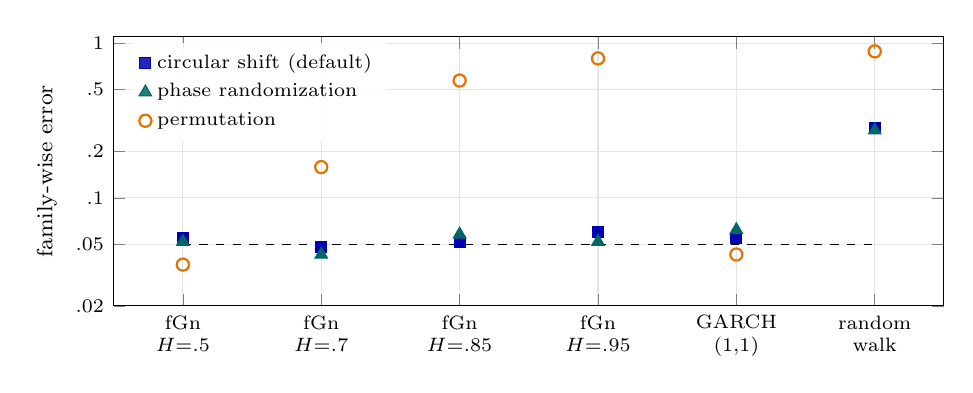
\begin{tikzpicture}
\begin{axis}[
  width=\columnwidth, height=5.0cm,
  ymode=log, ymin=0.02, ymax=1.1,
  ytick={0.02,0.05,0.1,0.2,0.5,1}, yticklabels={.02,.05,.1,.2,.5,1},
  symbolic x coords={W,H70,H85,H95,GARCH,RW},
  xtick=data,
  xticklabels={{fGn\\$H{=}.5$},{fGn\\$H{=}.7$},{fGn\\$H{=}.85$},{fGn\\$H{=}.95$},{GARCH\\(1,1)},{random\\walk}},
  xticklabel style={align=center,font=\scriptsize},
  yticklabel style={font=\scriptsize},
  ylabel={family-wise error}, ylabel style={font=\footnotesize},
  enlarge x limits=0.1,
  legend style={font=\scriptsize,at={(0.02,0.98)},anchor=north west,draw=none,fill=white,fill opacity=0.85,text opacity=1},
  legend cell align=left,
  grid=major, grid style={gray!20},
]
\addplot[only marks,mark=square*,mark size=2pt,color=blue!70!black] coordinates
  {(W,0.055) (H70,0.048) (H85,0.052) (H95,0.060) (GARCH,0.055) (RW,0.282)};
\addlegendentry{circular shift (default)}
\addplot[only marks,mark=triangle*,mark size=2.6pt,color=teal!80!black] coordinates
  {(W,0.052) (H70,0.043) (H85,0.058) (H95,0.052) (GARCH,0.062) (RW,0.273)};
\addlegendentry{phase randomization}
\addplot[only marks,mark=o,mark size=2.2pt,thick,color=orange!90!black] coordinates
  {(W,0.037) (H70,0.158) (H85,0.573) (H95,0.797) (GARCH,0.043) (RW,0.885)};
\addlegendentry{permutation}
\addplot[dashed,black,domain=0:1,forget plot] coordinates {(W,0.05) (RW,0.05)};
\end{axis}
\end{tikzpicture}
\caption{Null validity under dependent noise. Family-wise error of v2 rooting
on three independent channels, 400 trials per point, nominal 0.05 (dashed). The
two nulls that keep each series' memory hold size on every stationary process
tested. Permutation fails as soon as memory is long. Every null fails on random
walks, which are not stationary. Data: committed artifact
\code{dependent\_noise\_null\_study.json}.}
\label{fig:depnoise}
\end{figure}

Long memory costs power, as Prop.~\ref{prop:rev} predicts. With a 0.3 coupling
at lag 2 in fGn channels, circular-shift rooting recovered the true edge at its
true lag in 1.000, 0.990, 0.850, and 0.500 of 200 systems as $H$ rose from 0.5 to
0.95. Reverse edges rose from 0.000 to 0.105. This is the same reverse-lead
artifact as under AR(1) memory, now under power-law memory.

\subsection{Coherent oscillators and shared nonstationarity}

The preregistered phase and harmonic benchmark (configuration
\code{eebc6fbaaded\ldots}) tested rooting on held-out simulated channel pairs,
mostly of 2,048 samples, with 400 unrelated pairs per condition. Rooting held
size on independent oscillators at similar, 1:2, and 2:3 frequencies
(0.043--0.048) and on independent AR(0.95) pairs (0.058). It did not hold size in
the four conditions of Table~\ref{tab:coherent}.

\begin{table}[t]
\centering\footnotesize
\caption{False relationships on unrelated pairs. Rate of declared edges; 400
pairs per row; nominal .05. Bold: Wilson lower bound above .05. ``Gate'':
share of pairs on which the data-quality gate abstains.}
\label{tab:coherent}
\setlength{\tabcolsep}{3pt}
\begin{tabular}{@{}lcccc@{}}
\toprule
Independent pair & Rooting & Phase & No seam & Gate\\
\midrule
Identical frequency, coherent & \textbf{.145} & .040 & \textbf{.170} & --\\
Irregular timestamps & \textbf{.072} & .052 & .065 & --\\
Shared amplitude trend & \textbf{.150} & .037 & .060 & .072\\
Random walks & \textbf{.188} & .000 & .000 & 1.000\\
Shared 6--8\,Hz sweep & \textbf{.098} & \textbf{.077} & \textbf{.107} & .885\\
\bottomrule
\multicolumn{5}{p{0.95\columnwidth}}{\scriptsize ``Phase'': the experimental
$n{:}m$ phase-synchrony test, which uses an exact shift null corrected by a
linear phase ramp. ``No seam'': the same test without the ramp. Source:
\code{resonance\_math\_benchmark.json}.}
\end{tabular}
\end{table}

The coherent-oscillator row is the seam of Remark~\ref{rem:seam} made visible.
When two independent near-sinusoids share a frequency and $T$ is not a whole
number of periods, rotating a series breaks it at the seam, so surrogate
correlations run systematically lower than the observed correlation. The
experimental phase test removes the seam with a linear phase ramp that makes
the shifted phasor periodic, and it holds 0.040 on the same pairs. Its ablation
without the ramp rises to 0.170. This explains the apparent conflict with
Table~\ref{tab:size}, where rooting holds size on stochastic AR(2) oscillators
with $r=0.95$: a stochastic oscillator decorrelates within the record, and a
near-deterministic one does not.

The other rows are failures of stationarity, not of the seam. A shared trend or
frequency sweep makes independent series look aligned, and so do random walks.
The repository's data-quality gate abstains on every random-walk pair and on
88.5\% of shared sweeps, but on only 7.2\% of shared amplitude trends.
Detrending choices therefore remain the analyst's responsibility, and the null
cannot make them.

\subsection{Rooting against prewhitening-style baselines}

A paired robustness benchmark (configuration \code{691b9c61\ldots}, 200 trials
per case, three channels) compared v2 rooting under both nulls with
max-over-lags raw correlation and AR(1)-residual correlation. Both baselines use
thresholds calibrated on 399 separate white-noise trials. It is a fixed
exploratory benchmark, not a registered confirmatory study. Three findings bear
on this paper. First, raw correlation is unusable under long memory: its
white-noise threshold produced false alarms in 0.595 of fGn trials at $H=0.85$
and 0.900 at $H=0.95$. Second, residualizing helps power: at $H=0.95$ and
$c=0.3$, AR(1)-residual correlation found the injected edge in 1.000 of trials
against 0.535 for circular-shift rooting. However, with a white-noise threshold
its own false-alarm rate was 0.130 at $H=0.85$ and 0.095 at $H=0.95$. This is
the argument for v3, which prewhitens and then calibrates by resampling rather
than by a white-noise threshold. Third, at $H=0.95$ circular-shift rooting measured
0.090 [0.058, 0.138] here, against 0.060 [0.041, 0.088] in the dependent-noise
study. The designs differ in trial count and seeds, and the intervals overlap.
We treat $H=0.95$ as the edge of the tested validity region, not inside it.

\section{External Evidence: Three Preregistered Tests}\label{sec:external}

Table~\ref{tab:external} summarizes the three external tests. Each fixed its
data, holdout, baselines, decision rule, and tolerance before scoring. None
supported its claim.

\begin{table}[t]
\centering\footnotesize
\caption{Preregistered external tests. Every test reports every comparison,
including the ones that favored DRR.}
\label{tab:external}
\setlength{\tabcolsep}{3pt}
\begin{tabular}{@{}p{0.2\columnwidth}p{0.4\columnwidth}p{0.32\columnwidth}@{}}
\toprule
Test & Decisive outcome & Status\\
\midrule
NOAA QBO disruptions & Holdout false-alarm rate .272 vs.\ .05 tolerance; no unique hit & not\_supported (false-alarm rate)\\
\addlinespace
Daily crypto returns, 2023--25 & MSE gain .34\% vs.\ zero return, .08\% vs.\ ridge; Holm $p=1.0$ & not supported (2 of 5 gates failed)\\
\addlinespace
Lead--lag breakdown & Pooled delay 41.7 obs.\ worse than signed correlation; false-alarm gate failed & not supported (3 of 3 gates failed)\\
\bottomrule
\end{tabular}
\end{table}

\subsection{Quasi-biennial oscillation (claim not supported)}

The quasi-biennial oscillation (QBO) of equatorial stratospheric winds has a
period of about 28 months \cite{baldwin}. Two published disruptions occurred in
2016 \cite{osprey,newman} and 2019--2020 \cite{anstey}. The repository's
preregistration fixed the following before scoring: data checksums (NOAA CPC 30
and 50\,hPa indices, 1979-01 to 2026-08, 572 months); the disruption windows
taken from those papers; an 84-month trailing window; a holdout from 2011-01;
conventional detectors; spectral and rooting ablations; and a decision rule.
Each detector is calibrated to a 5\% false-alarm rate before 2011 and applied
unchanged afterwards. The claim was that full DRR flags disruptions that the
conventional detectors miss while keeping the holdout false-alarm rate at or
below 0.05.

\begin{table}[t]
\centering\footnotesize
\caption{Preregistered QBO comparison (committed artifact, reproduced exactly).
Claim status: not\_supported, reason \code{drr\_false\_alarm\_rate}.}
\label{tab:qbo}
\setlength{\tabcolsep}{3pt}
\begin{tabular}{@{}llccc@{}}
\toprule
Model & Role & Holdout FAR & 2016 & 2019--20\\
\midrule
Rolling volatility & conventional & .572 & hit & hit\\
Rolling correlation & conventional & .461 & hit & hit\\
VAR(1) residual & conventional & .072 & hit & miss\\
Regularized logistic & conventional & \multicolumn{3}{c}{withheld (no estimation labels)}\\
DRR spectral & ablation & .272 & miss & hit\\
DRR rooting & ablation & \multicolumn{3}{c}{uncalibrated (two-valued score)}\\
DRR full & DRR & .272 & miss & hit\\
\bottomrule
\end{tabular}
\end{table}

Full DRR alarmed on 27.2\% of quiet holdout months, against a tolerance of 0.05
(Table~\ref{tab:qbo}). It missed the 2016 disruption and had no detection that a
calibrated conventional detector missed. The block-bootstrap interval for unique
hits is [0, 0]. The claim is not supported. Every detector, conventional ones
included, exceeded its estimation-period false-alarm rate on the holdout. This
is consistent with a change in the series' behavior after 2011, but that
interpretation is conjecture, not a finding. The result is confined to
stratospheric wind and does not bear on DRR in any other domain.

\begin{figure*}[t]
\centering
\includegraphics[page=6,trim=40 606 46 46,clip,width=\textwidth]{\src}
\caption{QBO exploratory checks. (a) The two levels with the preregistered
disruption windows. (b) Raw levels are almost perfectly correlated across a wide
band of lags, as Prop.~\ref{prop:rev} predicts for narrowband signals. Prewhitened
innovations concentrate the association at lags 0 to 2 months.}
\label{fig:qbo}
\end{figure*}

\subsection{Exploratory known-answer checks of v3 operators}

The v3 operators were then applied to the same data. These checks were run
after the preregistered result was known, with settings frozen beforehand
(12-month maximum lag, 999 surrogates, AR order at most 12). They are
exploratory and do not change the claim status. A confirmatory v3 claim on the
QBO would need a new preregistration. The physics supplies a known answer: QBO
shear zones descend, so 30\,hPa should lead 50\,hPa \cite{baldwin}.

\textit{Rooting.} Both operators report the physical direction
(Fig.~\ref{fig:qbo}). v2 reports 30$\to$50\,hPa at lag 3 months ($\padj=0.001$),
and v3 reports it at lag 1 month ($\padj=0.002$). Neither is clean. The reverse
direction also passes the surrogate test in both: $\padj=0.008$ for v2 at lag 10,
and 0.027 for v3 at lag 1. It is excluded only by the heuristic candidate gate.
With two variables, that gate can decide an edge that the calibrated test does
not. We therefore recommend reporting every surrogate-tested edge and retiring
the gate. The residual reverse association in v3 is plausible given monthly
averaging of a process that descends about 1\,km per month, and it may reflect
contemporaneous forcing. We do not interpret it further. Monthly QBO levels are
also close to the coherent-oscillator case of Section~\ref{sec:nulls}, where the
v2 null is known to be anti-conservative. That is a further reason not to read
the v2 reverse edge as evidence.

\textit{Resonance.} The QBO is a textbook oscillation: bins 18--24 hold about half
of each level's variance. Yet $D^*$ does not reject its nulls ($p=0.81$ and
0.73 under AR(1); 0.29 and 0.20 under isotonic). Monthly sampling of a 28-month
cycle gives lag-1 autocorrelations of 0.95 (30\,hPa) and 0.94 (50\,hPa), and the
matched red null reproduces the depth. $\Lambda$ rejects $H_{\mathrm{mono}}$ at
both levels ($p=0.016$ at 50\,hPa; $p=0.008$ at 30\,hPa, 999 surrogates). At
50\,hPa the line sits at 27.2 months, the QBO. At 30\,hPa the QBO line (ratio
10.0) is second to a line at 2.0 months, next to the Nyquist frequency (ratio
16.7), whose origin we have not investigated. $\Lambda$ tests for a line;
locating it requires review.

\subsection{Daily cryptocurrency returns (claim not supported)}

The financial holdout (protocol \code{a106ed97380f\ldots}) asked whether DRR
features improve forecasts and cost-adjusted decisions relative to conventional
alternatives. Its design was locked in stages before scoring, with every
amendment logged. The target is the next-day open-to-open return on BTCUSDT and
ETHUSDT, with a full intervening day after the feature bar closes. Development
used 2018--2020 and selection used 2021--2022. The holdout is 1,096 entry dates
from 2023-01-01 to 2025-12-31. Baselines are zero return, the historical mean,
20-day momentum, ridge regression, and gradient boosting. Candidates are the
ridge and boosting models with DRR features added under identical tuning
budgets. Spectral-only, rooting-only, and random-noise feature sets serve as
controls. Validation selected ridge + DRR as the primary candidate, using mean
squared error, never holdout profit.

On the holdout, ridge + DRR had MSE $8.4385\times10^{-4}$, against
$8.4675\times10^{-4}$ for zero return and $8.4450\times10^{-4}$ for ridge, a
0.34\% and 0.08\% improvement. The protocol required at least 1\% against every
baseline and Holm-significant improvements at every bootstrap block length (7,
30, and 90 days) over a 14-test family. Both gates failed: against zero return,
historical mean, and ridge, every Holm-adjusted $p$ was 1.0. The candidate did
pass the other three gates: positive cumulative return at the stress cost of 30
basis points, wins over the zero-return comparator on MSE in two of three test years, and
at least 85\% interval coverage on each asset. All five had to pass. Boosting with DRR features was worse than zero return on
MSE. The verdict is \emph{not supported}. The data are public history rather
than a blind live trial, which the protocol records as a limitation.

\subsection{Lead--lag breakdown (claim not supported)}

The breakdown study (protocol \code{9fa1cdecb1a5\ldots}) asked whether a fixed
DRR fingerprint detects a breakdown in lead--lag structure sooner than
conventional detectors under the same calibrated false-alarm budget. The
fingerprint combines two directed max-absolute correlations with their lags
(Eq.~\eqref{eq:root}) and the depth components of each series. Baselines were a
signed-correlation monitor, VAR-residual CUSUM \cite{page}, and Bayesian online
change-point detection on VAR residuals \cite{adams}. Thresholds were calibrated
to a 5\% pathwise false-alarm budget on 64 independent paths per null
scenario. Each of
seven scenarios (no change, volatility-only shock, coupling drop, gradual drop,
reversal, lag shift, and a common driver) had 96 held-out paired replicates. The
first alarm was scored, and misses and early alarms took the full 256-observation
delay penalty.

All three success gates failed. Realized held-out false-alarm rates on the
unchanged scenario were not comparable across methods: 0\% for DRR, 7.3\% for
the spectral-only ablation, and 6.3\% for VAR change-point detection. Pooled
over the four true-change scenarios, DRR was 41.7 observations slower than
signed correlation (95\% CI $-51.9$ to $-31.9$). It was faster on coupling drops
(20.3 observations, Holm $p=0.030$) and gradual drops (16.3, $p=0.006$), but much
slower on reversals ($-158.0$) and lag shifts ($-45.3$). Signed correlation
detected 95.8\% of reversals, against 20.8\% for DRR and 39.6\% for its
rooting-only ablation. One plausible contributor is that the fingerprint's
correlations are sign-blind by construction, but this was not tested. DRR beat
both VAR detectors in all ten comparisons with them, which detected almost
nothing in this design. On held-out 2026 hourly market data, DRR issued 2
warnings in 531 eligible hours, too few for inference. The verdict is
\emph{not supported}.

\section{The Evidence Ledger}\label{sec:ledger}

DRR separates three layers: the operator core, a validation substrate, and
domain adapters. Claims are typed by evidence class:
\begin{itemize}
\item \emph{Specification}: the code does what the definition says (property
tests, and a JavaScript port checked against Python to $10^{-9}$).
\item \emph{Calibration}: error rates on systems with a known truth
(Sections~\ref{sec:calroot}--\ref{sec:nulls}).
\item \emph{External}: preregistered, hash-pinned tests on public data
(Section~\ref{sec:external}).
\end{itemize}
Each claim carries a machine-readable status. A universal claim concerns
operators, and a domain claim stays inside its adapter. Table~\ref{tab:ledger}
lists the current entries that this paper relies on.

\begin{table}[t]
\centering\footnotesize
\caption{Ledger entries cited in this paper. ``Sim.'': simulation evidence.
``Ext.'': external, preregistered.}
\label{tab:ledger}
\setlength{\tabcolsep}{2.5pt}
\begin{tabular}{@{}p{0.52\columnwidth}cp{0.3\columnwidth}@{}}
\toprule
Claim & Class & Status\\
\midrule
Thm.~\ref{thm:suff}, Props.~\ref{prop:exact}--\ref{prop:rev} & proof & proven\\
v2 rooting FWER on stationary AR, fGn ($H\le0.85$), GARCH & sim. & supported\\
v2 rooting FWER at fGn $H=0.95$ & sim. & borderline (two studies)\\
v2 rooting on coherent oscillators, trends, random walks & sim. & not controlled\\
v3 prewhitened rooting: size and exact-lag recovery & sim. & supported; outside package\\
$\Lambda$: size and power on 16 families & sim. & supported; addendum, outside package\\
Phase test: 1:2 and 2:3 coupling & sim. & supported (8 of 9 hyp.)\\
Phase test: 1:1 non-inferiority to rooting & sim. & not supported\\
DRR-Mellin recovery superiority & sim. & partially supported\\
QBO disruption detection & ext. & not\_supported\\
Daily crypto-return forecasting & ext. & not supported\\
Lead--lag breakdown detection & ext. & not supported\\
Earlier financial-stress lead times, AUROC & -- & withdrawn\\
\bottomrule
\end{tabular}
\end{table}

The ledger has now recorded three external failures rather than dropping them.
Earlier repository documents had carried lead-time and AUROC figures for
financial-stress episodes that no code in the repository produced. Those
figures are recorded as withdrawn, with their history preserved. Two entries
outside this paper's main line are listed because they share its discipline.
The phase-synchrony test detected 1:2 and 2:3 coupling in 28.0--35.5\% of
held-out pairs, where rooting detected 2.5--5.0\%, but it was weaker than rooting
for ordinary 1:1 coupling (mean 0.263 vs.\ 0.441). The DRR-Mellin log-frequency
scan recovered off-grid log-periodic modes less often than Lomb--Scargle
\cite{lomb,scargle} and nonlinear least squares when pooled over 12,000 held-out
records (0.666 vs.\ 0.694 and 0.688), and more often than ESPRIT \cite{esprit}
(0.392). It was the most reliable method for strongly growing or decaying
envelopes in additive noise, and lost under scale-proportional noise, as
predicted. In the vocabulary of model-risk guidance \cite{sr117}, the theorems
and specification tests address conceptual soundness, the calibration studies
address implementation and limits, and the preregistered tests are outcomes
analysis. None of it substitutes for independent validation for a specific
intended use.

\section{Discussion}

\textit{What DRR now is.} DRR consists of two calibrated tests and a descriptive
score, each with a known error profile and now a mapped validity region.
Rooting is a family-wise-controlled, lag-localized lead--lag screen. Its power
matches Granger in linear settings, and its null holds on stationary processes
with short or moderately long memory and heavy-tailed volatility. $\Lambda$ is a
size-robust test for spectral lines above any monotone continuum. Depth,
reported as $D^*$, says how rhythmic a trace is relative to memory, not whether
it is. The pieces are standard: surrogates, red-noise nulls, isotonic regression,
and prewhitening. What is new is the theorem that ties depth to the spectrum and
the resulting redefinition of resonance. Also new is the explicit composition of
these pieces under one ledger in which failures are first-class results.

\textit{What it is not.} Rooting is pairwise. A common driver of two channels
creates edges that no pairwise method can reject. In the breakdown study, a
common driver triggered DRR alarms in 62.5\% of replicates. Conditioning sets as
in PCMCI \cite{pcmci} are the natural next step. The rooting null is not valid
for near-deterministic oscillators that share a frequency, for shared trends, or
for integrated series. Each of these needs a seam correction, detrending, or
differencing chosen and justified by the analyst. Thm.~\ref{thm:suff} is a
statement about Gaussian processes. Non-Gaussian phase structure (for example,
intermittent bursts) is exactly where depth's phase and amplitude components
could carry information beyond the spectrum, and that remains untested. The
fitted-null bootstrap is not exact, which is why size was measured. The
transfer-entropy backend has no calibration yet.

\textit{What the external record says.} Three preregistered tests on two kinds of
data did not support their claims. The failures differ. The QBO test failed on
false alarms under an apparent change in the series after 2011. The return
forecast failed because DRR features added almost nothing to a ridge model. The
breakdown study failed because a simpler signed statistic was faster on the
changes that matter most. For these targets, the record is consistent with DRR
features carrying little incremental information beyond conventional baselines.
It does not show that DRR is uninformative elsewhere, and it does not yet show
that DRR adds information on real data anywhere. Every positive result in this paper is simulation
evidence.

\textit{Limitations.} There is no confirmatory external evidence for any
operator. The v3 operators (prewhitened rooting and $\Lambda$) are not yet in
the package, and their study scripts accompany this manuscript rather than the
repository. The simulation studies choose families that stress known failure
modes and cannot cover every realistic process. $\Lambda$ is a line detector and
does not detect broad peaks at $T=512$. The QBO 30\,hPa line near the Nyquist
frequency is unexplained. The $\Lambda$ statistic was added after the first study
run showed that $D^*$ lacked power in red noise. That design iteration is
recorded in the addendum configuration, and the $\Lambda$ results are simulation
evidence, not a confirmatory claim. The dependent-noise and robustness studies
tested v2 rooting only, so the size of v3 under long memory and coherent
oscillation is unknown.

\textit{Next steps.} (1) Move the v3 operators into the package behind version
flags (\code{rooting\_v3}, \code{resonance\_test\_v1}), with their study scripts
and calibration in CI. (2) Rerun the dependent-noise and coherent-oscillator
designs on v3, and add a seam correction to the rooting null (a phase ramp or
tapered shifts), adopting it only if a size study supports it. (3) Retire the
heuristic candidate gate, report every surrogate-tested edge, and add signed
lags to the rooting output. (4) Add conditional rooting. (5) Preregister a v3
external test on a dataset not yet examined. That preregistration should record
data checksums, event windows from the literature, holdout, tolerance,
baselines including a red-noise spectral test, Granger, and a signed-correlation
monitor, ablations, and the decision rule, under a new protocol ID.

\section{Conclusion}

DRR asks readers to check error rates rather than trust definitions. The rooting
test holds its family-wise error at the nominal level on the stationary
processes tested, including long memory and GARCH noise. It fails on coherent
oscillators, shared trends, and random walks, and we now know why. Its lead--lag
estimator failed under memory. The reason is derived in closed form, and the fix
restores power without giving up size. Resonance depth could not separate rhythm
from memory, and a theorem now explains why. Resonance is redefined so that the
distinction becomes a test with measured size and power. The framework's three
preregistered external claims all failed and are reported as such. A method that
publishes where it breaks, with the scripts that break it, is a stronger
foundation than one that does not.

\medskip
\noindent\textit{Data and code availability.} Code for the operators and all
committed studies is at
\url{https://github.com/topherchris420/dynamic-resonance-rooting} (MIT). The v3
study scripts, configurations, and JSON artifacts accompany this manuscript
(Appendix). The QBO data are U.S. government work from NOAA CPC, vendored with
checksums. The market data are from Binance Vision and are used under its
dataset terms (CC BY-NC-SA 4.0).

\section*{Appendix: Reproduction}

\textit{v3 study environment.} Python 3.11.15, NumPy 2.4.4, SciPy 1.17.1,
scikit-learn 1.8.0, drr-framework 4.3.0 at commit \code{862c4f7}. Running
\code{python run\_study.py} (configuration SHA-256 \code{57d5ea78f1c8\ldots5cb7},
33 tasks, about 25 min on two cores) writes \code{results/study.json}. Running
\code{python run\_spectral\_excess.py} (addendum configuration SHA-256
\code{b92f522f3472\ldots2de5}) writes \code{results/spectral\_excess.json}, and
\code{python make\_figures.py} renders Figs.~\ref{fig:rooting}, \ref{fig:resonance},
and~\ref{fig:qbo} from those files. Seeds: 20260925 (study), 20260926 (addendum). Every value in
Tables~\ref{tab:prop2}--\ref{tab:res} is read from these artifacts or from the
committed repository artifacts.

\textit{Committed evidence.} Values in Sections~\ref{sec:nulls}
and~\ref{sec:external} and Fig.~\ref{fig:depnoise} are read from artifacts under
\code{results/expected/} at repository commit \code{0f4f5f3}. Each regenerates
from a script in \code{scripts/}:
\code{run\_calibration\_study.py} and \code{run\_structural\_change\_benchmark.py}
(Tables~\ref{tab:size} v2 column and~\ref{tab:qbo});
\code{run\_dependent\_noise\_study.py} (config \code{b0a4cbc2a80e\ldots});
\code{run\_robustness\_benchmark.py} (config \code{691b9c618413\ldots});
\code{run\_resonance\_math\_benchmark.py} (config \code{eebc6fbaaded\ldots});
\code{run\_mellin\_recovery\_benchmark.py} (preregistration \code{a6fbf4ed6de4\ldots});
\code{run\_financial\_holdout.py} (protocol \code{a106ed97380f\ldots}); and
\code{run\_breakdown\_study.py} (protocol \code{9fa1cdecb1a5\ldots}, lock
\code{51fdcfd0e7b9\ldots}). The rendered Markdown reports beside each JSON
artifact list every row, including those not quoted here. The two market
studies verify their sealed ledgers by replay with platform-tolerant numerical
comparison.

\footnotesize
\begin{thebibliography}{99}\setlength{\itemsep}{0pt}
\bibitem{holland} J.~H. Holland, \emph{Adaptation in Natural and Artificial Systems}. Cambridge, MA: MIT Press, 1992.
\bibitem{mitchell} M.~Mitchell, \emph{Complexity: A Guided Tour}. New York: Oxford Univ. Press, 2009.
\bibitem{ditlevsen} P.~D. Ditlevsen and S.~J. Johnsen, ``Tipping points: Early warning and wishful thinking,'' \emph{Geophys. Res. Lett.}, vol.~37, L19703, 2010.
\bibitem{boettiger} C.~Boettiger and A.~Hastings, ``Quantifying limits to detection of early warning for critical transitions,'' \emph{J. R. Soc. Interface}, vol.~9, no.~75, pp.~2527--2539, 2012.
\bibitem{drr} C.~Woodyard, \emph{Dynamic Resonance Rooting} (software), v4.3.0, commits 862c4f7 (v3 study) and 0f4f5f3 (committed evidence), 2026. [Online]. Available: \url{https://github.com/topherchris420/dynamic-resonance-rooting}
\bibitem{theiler} J.~Theiler, S.~Eubank, A.~Longtin, B.~Galdrikian, and J.~D. Farmer, ``Testing for nonlinearity in time series: The method of surrogate data,'' \emph{Physica D}, vol.~58, pp.~77--94, 1992.
\bibitem{schreiber} T.~Schreiber and A.~Schmitz, ``Surrogate time series,'' \emph{Physica D}, vol.~142, pp.~346--382, 2000.
\bibitem{lancaster} G.~Lancaster, D.~Iatsenko, A.~Pidde, V.~Ticcinelli, and A.~Stefanovska, ``Surrogate data for hypothesis testing of physical systems,'' \emph{Phys. Rep.}, vol.~748, pp.~1--60, 2018.
\bibitem{gilman} D.~L. Gilman, F.~J. Fuglister, and J.~M. Mitchell, ``On the power spectrum of `red noise','' \emph{J. Atmos. Sci.}, vol.~20, pp.~182--184, 1963.
\bibitem{mannlees} M.~E. Mann and J.~M. Lees, ``Robust estimation of background noise and signal detection in climatic time series,'' \emph{Climatic Change}, vol.~33, pp.~409--445, 1996.
\bibitem{torrence} C.~Torrence and G.~P. Compo, ``A practical guide to wavelet analysis,'' \emph{Bull. Amer. Meteor. Soc.}, vol.~79, pp.~61--78, 1998.
\bibitem{burg} J.~P. Burg, ``Maximum entropy spectral analysis,'' Ph.D. dissertation, Stanford Univ., 1975.
\bibitem{barlow} R.~E. Barlow, D.~J. Bartholomew, J.~M. Bremner, and H.~D. Brunk, \emph{Statistical Inference Under Order Restrictions}. New York: Wiley, 1972.
\bibitem{anevski} D.~Anevski and P.~Soulier, ``Monotone spectral density estimation,'' \emph{Ann. Statist.}, vol.~39, no.~1, pp.~418--438, 2011.
\bibitem{mandelbrot} B.~B. Mandelbrot and J.~W. Van~Ness, ``Fractional Brownian motions, fractional noises and applications,'' \emph{SIAM Rev.}, vol.~10, no.~4, pp.~422--437, 1968.
\bibitem{daviesharte} R.~B. Davies and D.~S. Harte, ``Tests for Hurst effect,'' \emph{Biometrika}, vol.~74, no.~1, pp.~95--101, 1987.
\bibitem{bollerslev} T.~Bollerslev, ``Generalized autoregressive conditional heteroskedasticity,'' \emph{J. Econometrics}, vol.~31, no.~3, pp.~307--327, 1986.
\bibitem{grangernewbold} C.~W.~J. Granger and P.~Newbold, ``Spurious regressions in econometrics,'' \emph{J. Econometrics}, vol.~2, no.~2, pp.~111--120, 1974.
\bibitem{granger} C.~W.~J. Granger, ``Investigating causal relations by econometric models and cross-spectral methods,'' \emph{Econometrica}, vol.~37, no.~3, pp.~424--438, 1969.
\bibitem{bartlett} M.~S. Bartlett, ``Some aspects of the time-correlation problem in regard to tests of significance,'' \emph{J. R. Statist. Soc.}, vol.~98, no.~3, pp.~536--543, 1935.
\bibitem{boxjenkins} G.~E.~P. Box and G.~M. Jenkins, \emph{Time Series Analysis: Forecasting and Control}, rev. ed. San Francisco: Holden-Day, 1976.
\bibitem{haugh} L.~D. Haugh, ``Checking the independence of two covariance-stationary time series: A univariate residual cross-correlation approach,'' \emph{J. Amer. Statist. Assoc.}, vol.~71, no.~354, pp.~378--385, 1976.
\bibitem{pcmci} J.~Runge, P.~Nowack, M.~Kretschmer, S.~Flaxman, and D.~Sejdinovic, ``Detecting and quantifying causal associations in large nonlinear time series datasets,'' \emph{Sci. Adv.}, vol.~5, no.~11, eaau4996, 2019.
\bibitem{westfall} P.~H. Westfall and S.~S. Young, \emph{Resampling-Based Multiple Testing}. New York: Wiley, 1993.
\bibitem{rosenblum} M.~G. Rosenblum, A.~S. Pikovsky, and J.~Kurths, ``Phase synchronization of chaotic oscillators,'' \emph{Phys. Rev. Lett.}, vol.~76, no.~11, pp.~1804--1807, 1996.
\bibitem{scheffer} M.~Scheffer \emph{et al.}, ``Early-warning signals for critical transitions,'' \emph{Nature}, vol.~461, pp.~53--59, 2009.
\bibitem{dakos} V.~Dakos \emph{et al.}, ``Methods for detecting early warnings of critical transitions in time series illustrated using simulated ecological data,'' \emph{PLoS ONE}, vol.~7, no.~7, e41010, 2012.
\bibitem{nosek} B.~A. Nosek, C.~R. Ebersole, A.~C. DeHaven, and D.~T. Mellor, ``The preregistration revolution,'' \emph{Proc. Natl. Acad. Sci. USA}, vol.~115, no.~11, pp.~2600--2606, 2018.
\bibitem{sr117} Board of Governors of the Federal Reserve System and Office of the Comptroller of the Currency, ``Supervisory guidance on model risk management,'' SR Letter 11-7, 2011.
\bibitem{welch} P.~Welch, ``The use of fast Fourier transform for the estimation of power spectra,'' \emph{IEEE Trans. Audio Electroacoust.}, vol.~15, no.~2, pp.~70--73, 1967.
\bibitem{gabor} D.~Gabor, ``Theory of communication,'' \emph{J. IEE}, vol.~93, no.~26, pp.~429--457, 1946.
\bibitem{hemerik} J.~Hemerik and J.~Goeman, ``Exact testing with random permutations,'' \emph{TEST}, vol.~27, pp.~811--825, 2018.
\bibitem{lehmann} E.~L. Lehmann and J.~P. Romano, \emph{Testing Statistical Hypotheses}, 3rd ed. New York: Springer, 2005.
\bibitem{brockwell} P.~J. Brockwell and R.~A. Davis, \emph{Time Series: Theory and Methods}, 2nd ed. New York: Springer, 1991.
\bibitem{akaike} H.~Akaike, ``A new look at the statistical model identification,'' \emph{IEEE Trans. Autom. Control}, vol.~19, no.~6, pp.~716--723, 1974.
\bibitem{wilson} E.~B. Wilson, ``Probable inference, the law of succession, and statistical inference,'' \emph{J. Amer. Statist. Assoc.}, vol.~22, no.~158, pp.~209--212, 1927.
\bibitem{baldwin} M.~P. Baldwin \emph{et al.}, ``The quasi-biennial oscillation,'' \emph{Rev. Geophys.}, vol.~39, no.~2, pp.~179--229, 2001.
\bibitem{osprey} S.~M. Osprey \emph{et al.}, ``An unexpected disruption of the atmospheric quasi-biennial oscillation,'' \emph{Science}, vol.~353, no.~6306, pp.~1424--1427, 2016.
\bibitem{newman} P.~A. Newman, L.~Coy, S.~Pawson, and L.~R. Lait, ``The anomalous change in the QBO in 2015--2016,'' \emph{Geophys. Res. Lett.}, vol.~43, pp.~8791--8797, 2016.
\bibitem{anstey} J.~A. Anstey \emph{et al.}, ``Prospect of increased disruption to the QBO in a changing climate,'' \emph{Geophys. Res. Lett.}, vol.~48, e2021GL093058, 2021.
\bibitem{page} E.~S. Page, ``Continuous inspection schemes,'' \emph{Biometrika}, vol.~41, no.~1/2, pp.~100--115, 1954.
\bibitem{adams} R.~P. Adams and D.~J.~C. MacKay, ``Bayesian online changepoint detection,'' arXiv:0710.3742, 2007.
\bibitem{lomb} N.~R. Lomb, ``Least-squares frequency analysis of unequally spaced data,'' \emph{Astrophys. Space Sci.}, vol.~39, pp.~447--462, 1976.
\bibitem{scargle} J.~D. Scargle, ``Studies in astronomical time series analysis. II. Statistical aspects of spectral analysis of unevenly spaced data,'' \emph{Astrophys. J.}, vol.~263, pp.~835--853, 1982.
\bibitem{esprit} R.~Roy and T.~Kailath, ``ESPRIT---Estimation of signal parameters via rotational invariance techniques,'' \emph{IEEE Trans. Acoust., Speech, Signal Process.}, vol.~37, no.~7, pp.~984--995, 1989.
\end{thebibliography}

\end{document}
